\chapter{Plotting Examples Using Different Programs} 
\label{cha:evaluation}

\section{Plotting with tikz}

See the example \figref{fig:tikz_example_01}
\begin{figure}[ht]
    \centering
    \begin{center}

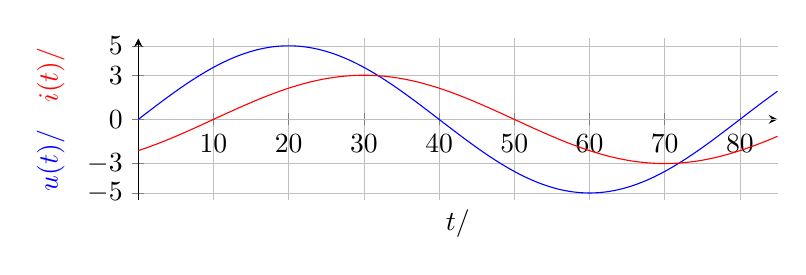
\begin{tikzpicture}
    \begin{axis}[
        domain=0:85,
        xmin=0, xmax=85,
        ymin=-5.5, ymax=5.5,
        samples=500,
        axis y line=center,
        axis x line=middle,
        xtick distance=10,
        ytick distance=1,
        extra y ticks=0,
        width=.8\textwidth,
        height=.3\textwidth,
        x label style={at={(axis description cs:0.5,0)},anchor=north},
        y label style={at={(axis description cs:-.1,.5)},rotate=90,anchor=south},
        ytick={-5,-3,0,3,5},
%         yticklabels={$-2 u_0$, $2 u_0$},
        xlabel={$t/\ms$},
         ylabel={{\color{blue}$u(t)/\volt$}\quad{\color{red}$i(t)/\ampere$}},
        grid=both,
        grid style={line width=.1pt, draw=gray!10},
        major grid style={line width=.2pt,draw=gray!50}    ]
        \addplot+[color=blue,mark=none] {5*sin(deg(x/80*6.283))};
        \addplot+[color=red,mark=none] {3*sin(deg((x-10)/80*6.283))};
    \end{axis}
\end{tikzpicture}
\end{center}
    \caption{Example of a tikz figure}
    \label{fig:tikz_example_01}
\end{figure}
\begin{figure}[ht]
    \centering
    \begin{center}
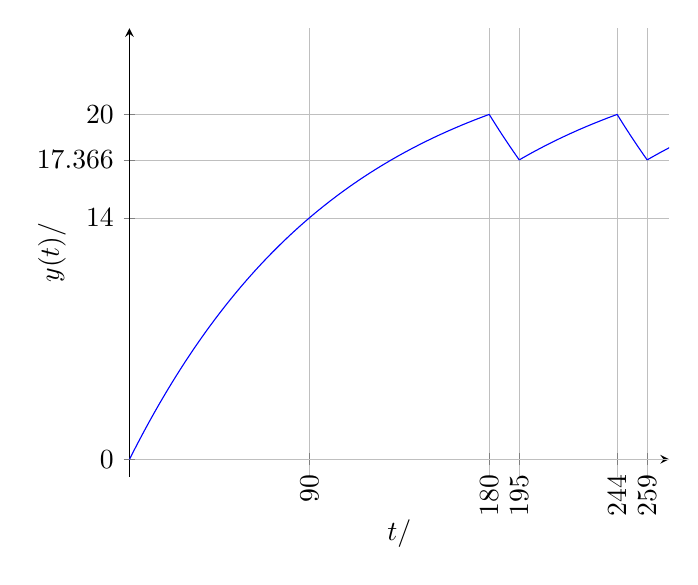
\begin{tikzpicture}
    \begin{axis}[
        domain=0:270,
        xmin=0, xmax=270,
        ymin=-1, ymax=25,
        samples=500,
        axis y line=center,
        axis x line=middle,
        %xtick distance=1,
        %ytick distance=1,
        extra y ticks=0,
        x label style={at={(axis description cs:0.5,-.075)},anchor=north},
        y label style={at={(axis description cs:-.1,.5)},rotate=90,anchor=south},
        xlabel={$t/\minute$},
        ylabel={$y(t)/\celsius$},
        ytick={0,14,17.366,20},
        xtick={0, 90, 180, 195,  244,  259},
        xticklabels={0, 90, 180, 195,  244,  259},
        xticklabel style={rotate=90},
        yticklabels={0,14,17.366,20},
        grid=both,
        grid style={line width=.1pt, draw=gray!10},
        major grid style={line width=.2pt,draw=gray!50},    ]
        \addplot+[color=blue,mark=none,domain=0:180] {2000*0.01225*(1-exp(-x/106.22))};
        \addplot+[color=blue,mark=none,domain=180:195] {20*(exp(-(x-180)/106.22))};
        \addplot+[color=blue,mark=none,domain=195:244] {2000*0.01225*(1-exp(-(x-64)/106.22))};
        \addplot+[color=blue,mark=none,domain=244:259] {20*(exp(-(x-244)/106.22))};
        \addplot+[color=blue,mark=none,domain=259:300] {2000*0.01225*(1-exp(-(x-128)/106.22))};
    \end{axis}
\end{tikzpicture}
\end{center}
    \caption{Example of another tikz figure}
    \label{fig:tikz_example_02}
\end{figure}
\begin{figure}[ht]
    \centering
    \begin{center}
\begin{tikzpicture}
    \begin{axis}[
        domain=0:300,
        xmin=0, xmax=300,
        ymin=-1, ymax=2200,
        samples=500,
        axis y line=center,
        axis x line=middle,
        %xtick distance=1,
        %ytick distance=1,
        extra y ticks=0,
        x label style={at={(axis description cs:0.5,-.075)},anchor=north},
        y label style={at={(axis description cs:-.1,.5)},rotate=90,anchor=south},
        xlabel={$t/\minute$},
        ylabel={$u(t)/\watt$},
        xtick={0, 90, 180, 195,  244,  259},
        xticklabels={0, 90, 180, 195,  244,  259},
        xticklabel style={rotate=90},
        ytick={0,2000},
        yticklabels={0,2000},
        %yticklabels={$-2 u_0$,$-u_0$, $0$,$\frac{u_0}{2}$, $u_0$},
        grid=both,
        grid style={line width=.1pt, draw=gray!10},
        major grid style={line width=.2pt,draw=gray!50},    ]
        \addplot[color=blue,mark=none] coordinates{
            ( 0,  2000)
            (180,  2000)
            (180,  0)
            (195,  0)
            (195,  2000)
            (244,  2000)
            (244,  0)
            (259,  0)
            (259,  2000)
            (300,  2000)
    };
    \end{axis}
\end{tikzpicture}
\end{center}
    \caption{Example of even another tikz figure}
    \label{fig:tikz_example_03}
\end{figure}



\section{Circuits with circuitikz}
\figref{fig:circuitikz_example} is fully drawn by \LaTeX code. Go to the code to see how this figure is created.
\begin{figure}[ht]
    \centering
    \begin{center}
\begin{circuitikz}
	\draw
	(0,0)
	to [short,o-*] ++(0,-.5) coordinate(up1) 
	(up1) to [short,-] ++(-1,0)  coordinate(up1l) 
	(up1) to [short,-] ++(1,0)  coordinate(up1r)
	(up1) ++(0,-2) coordinate(mid1o)
	(mid1o) to [short,-] ++(-1,0)  coordinate(mid1ol) 
	(mid1o) to [short,-] ++(1,0)  coordinate(mid1or)
	(mid1o) to [short,*-*] ++(0,-.5) coordinate(mid1u) 
	(mid1u) ++(0,-2) coordinate(down1)
	(mid1u) to [short,-] ++(-1,0)  coordinate(mid1ul) 
	(mid1u) to [short,-] ++(1,0)  coordinate(mid1ur)
	(down1) to [short,-] ++(-1,0)  coordinate(down1l) 
	(down1) to [short,-]  ++(1,0)  coordinate(down1r)
	(down1) to [short,*-o] ++(0,-.5) 
	(up1l) to [L,l^=$L$,v=$U_\text{L}$,mirror] (mid1ol)
	(up1r) to [R=$R$] (mid1or)
	(mid1ul) to [C,l_=$C$] (down1l)
	(mid1ur) to [R=$R$] (down1r)

        (5,0)
	to [short,o-*] ++(0,-.5) coordinate(up2) 
	(up2) to [short,-] ++(-1,0)  coordinate(up2l) 
	(up2) to [short,-] ++(1,0)  coordinate(up2r)
	(up2) ++(0,-4) coordinate(down2)
	(down2) to [short,-] ++(-1,0)  coordinate(down2l) 
	(down2) to [short,-]  ++(1,0)  coordinate(down2r)
	(down2) to [short,*-o] ++(0,-.5) 
	(up2l) to [R,l^=$R$,i=$i_\text{R}$] ++(0,-2) to  [C,l_=$C$] (down2l)
	(up2r) to [R=$R$] ++(0,-2) to [L,l^=$L$] (down2r)
	;
\end{circuitikz}

\end{center}

    \caption{Example of a circuitikz figure}
    \label{fig:circuitikz_example}
\end{figure}

\section{Circuits with Inkscape Library}
There is an Inkscape template for power electronics symbols provided by LEA, hosted on Github. \href{https://github.com/upb-lea/Inkscape_electric_Symbols}{https://github.com/upb-lea/Inkscape\_electric\_Symbols}. An overview is shown in \figref{fig:inkscape_example}. The included figure is a pdf-file, what is generated before by an Inkscape drawing.
\\ \\
Note: Preference should be given to vector graphics (e.g. PDF), as the image quality is much better than pixel graphics (e.g. JPG, PNG).

\begin{figure}[ht]
	\centering
    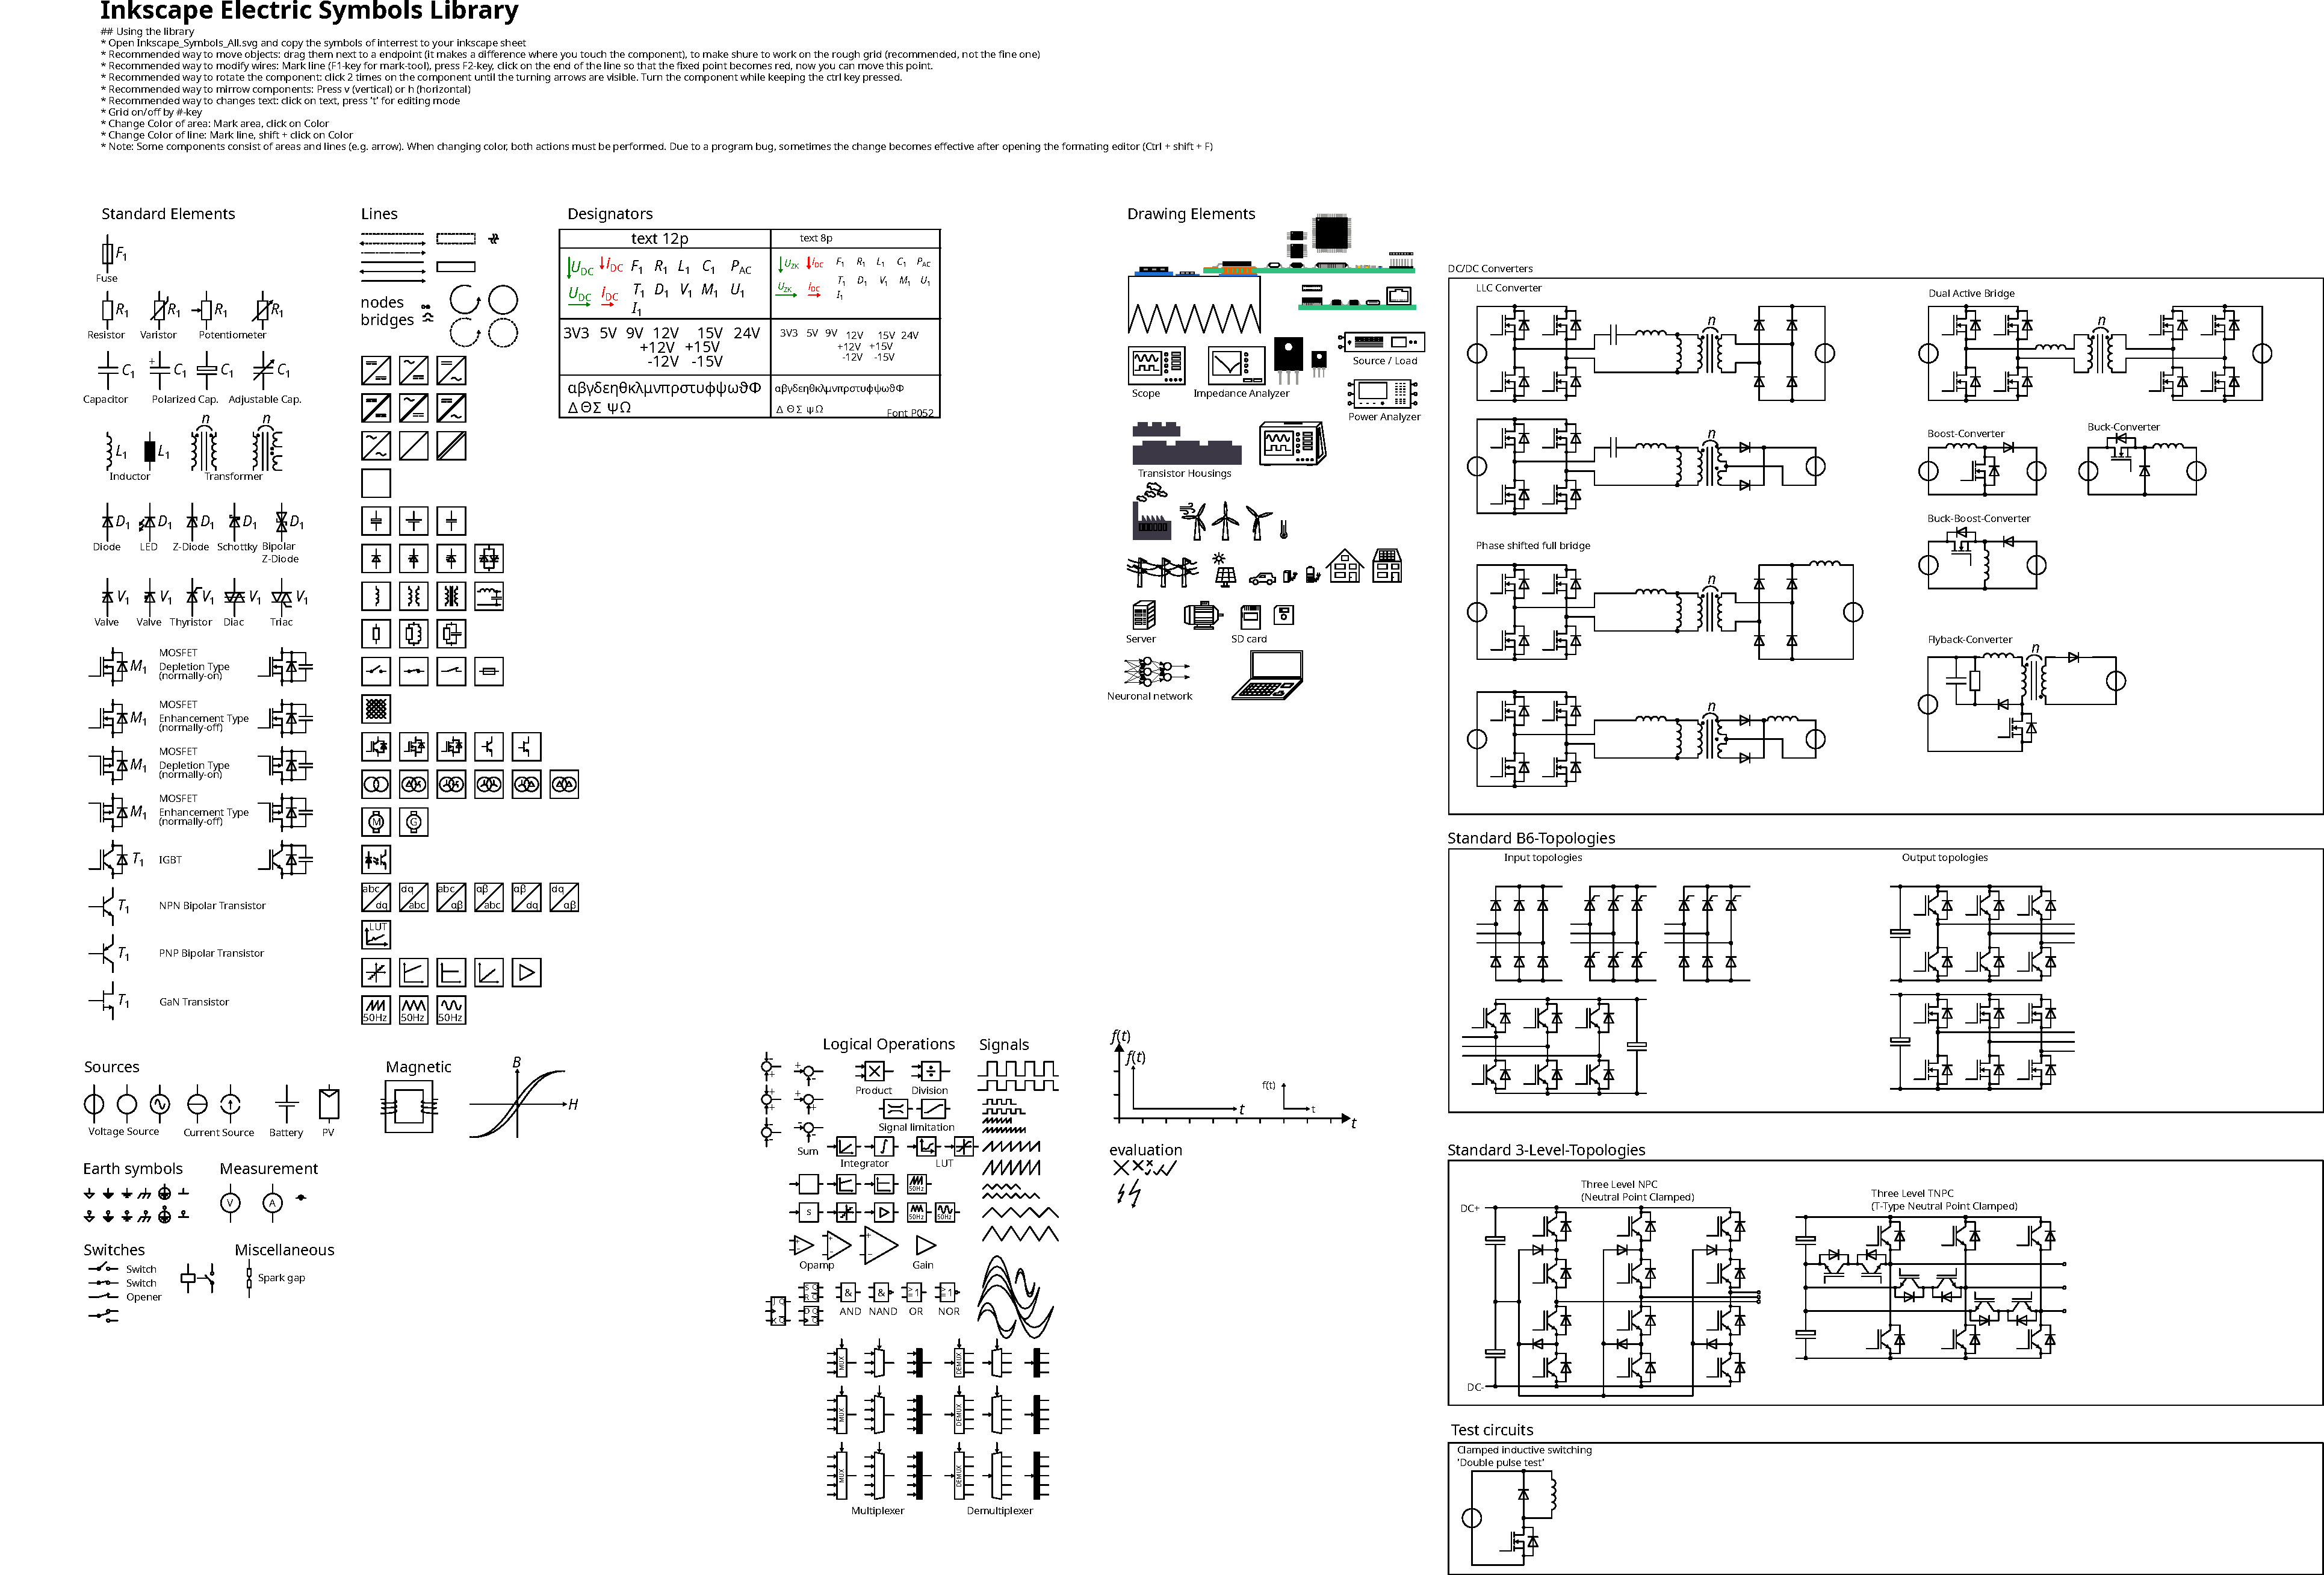
\includegraphics[]{fig/inkscape/Inkscape_Symbols_All.pdf}
	\caption{Example of a Inkscape figure}
	\label{fig:inkscape_example}
\end{figure}

